\chapter{Razões trigonométricas}

\section{Revisão}

Podemos identificar alguns elementos importantes num triângulo retângulo como, por exemplo, os catetos e a hipotenusa.

A hipotenusa é o lado que se opõe ao ângulo de $\SI{90}{\degree}$ (também conhecido como ângulo "reto") no triângulo retângulo.

Os catetos são os lados que não são hipotenusa.

Na figura abaixo, \textcolor{red!80}{$b$} é hipotenusa e \textcolor{blue!80}{$a$} e \textcolor{blue!80}{$c$} são catetos.

\begin{tikzscale}[0.8]
	\tkzDefPoints{0/0/A,4/0/B,4/3/C}
	\tkzDrawSegments[blue](A,B B,C)
	\tkzDrawSegment[red](A,C)

	\tkzLabelSegment[below=2pt, xshift=3pt, blue](A,B){$b$}
	\tkzLabelSegment[right=2pt, yshift=-2pt, blue](B,C){$a$}
	\tkzLabelSegment[above left, red](A,C){$c$}

	\tkzMarkRightAngle[line width=0.3pt](A,B,C)
	\tkzLabelAngle[pos=0.15](A,B,C){\small$\cdot$}

\end{tikzscale}

\section{Teorema de pitágoras}

\noindent Vale lembrar também o teorema de pitágoras, que estabelece que a soma do quadrado dos catetos é igual ao quadrado da hipotenusa, ou, em notação:

$$
	a^2+b^2=c^2
$$

Abaixo seguem duas provas desse fato, junto de suas visualizações geométricas.

\subsection{1ª demonstração}

\begin{multicols}{2}
	\noindent Como os triângulos são semelhantes a razão entre a área de um deles e da sua hipotenusa ao quadrado é constante:

	$$\frac{A_1}{\ell_1^2}=\frac{A_2}{\ell_2^2}=\frac{A_3}{\ell_3^2}=r$$

	\begin{center}
	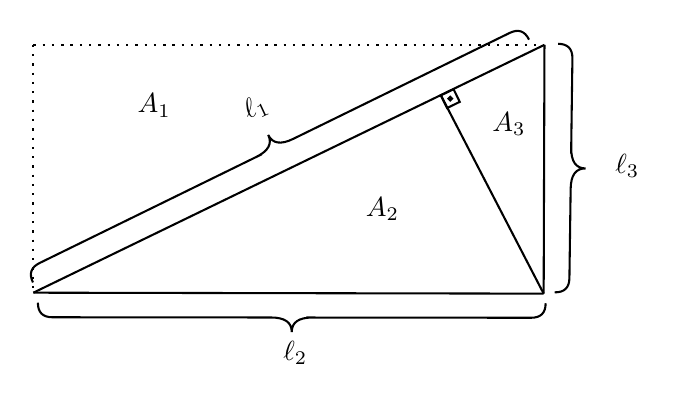
\begin{tikzpicture}[x=0.75pt,y=0.75pt,yscale=-1,xscale=1]

		\tikzset{every picture/.style={line width=0.75pt}} %set default line width to 0.75pt 

		%uncomment if require: \path (0,300); %set diagram left start at 0, and has height of 300

		%Straight Lines [id:da6702557414493615] 
		\draw    (390.07,59.75) -- (143.84,179.17) ;


		%Straight Lines [id:da9582819203019236] 
		\draw    (390.07,59.75) -- (389.68,179.63) ;


		%Straight Lines [id:da5632250014930594] 
		\draw    (143.84,179.17) -- (389.68,179.63) ;


		%Straight Lines [id:da6405899873814225] 
		\draw  [dash pattern={on 0.84pt off 2.51pt}]  (143.84,59.75) -- (143.84,179.17) ;


		%Straight Lines [id:da34190307039802803] 
		\draw  [dash pattern={on 0.84pt off 2.51pt}]  (143.84,59.75) -- (390.07,59.75) ;


		%Straight Lines [id:da6841177345207508] 
		\draw    (340.16,84.1) -- (389.68,179.63) ;


		%Shape: Square [id:dp8431878844102821] 
		\draw   (340.16,84.1) -- (346.27,81.12) -- (349.25,87.23) -- (343.15,90.21) -- cycle ;
		%Shape: Circle [id:dp4504121878155989] 
		\draw  [fill={rgb, 255:red, 0; green, 0; blue, 0 }  ,fill opacity=1 ] (345.56,85.66) .. controls (345.56,85.2) and (345.18,84.82) .. (344.71,84.82) .. controls (344.24,84.82) and (343.86,85.2) .. (343.86,85.66) .. controls (343.86,86.13) and (344.24,86.51) .. (344.71,86.51) .. controls (345.18,86.51) and (345.56,86.13) .. (345.56,85.66) -- cycle ;
		%Shape: Brace [id:dp8167678437120856] 
		\draw   (146,184) .. controls (145.99,188.67) and (148.32,191) .. (152.99,191.01) -- (258.31,191.12) .. controls (264.98,191.13) and (268.31,193.46) .. (268.3,198.13) .. controls (268.31,193.46) and (271.64,191.13) .. (278.31,191.14)(275.31,191.14) -- (383.63,191.25) .. controls (388.3,191.26) and (390.63,188.93) .. (390.63,184.26) ;
		%Shape: Brace [id:dp8291844918455844] 
		\draw   (395,179) .. controls (399.67,179.07) and (402.03,176.77) .. (402.09,172.1) -- (402.68,129.22) .. controls (402.77,122.55) and (405.14,119.25) .. (409.81,119.32) .. controls (405.14,119.25) and (402.86,115.89) .. (402.95,109.22)(402.91,112.22) -- (403.53,66.34) .. controls (403.6,61.68) and (401.3,59.32) .. (396.63,59.25) ;
		%Shape: Brace [id:dp7586079650511318] 
		\draw   (382.63,57.25) .. controls (380.58,53.06) and (377.46,51.99) .. (373.27,54.04) -- (269.03,105.06) .. controls (263.04,107.99) and (259.02,107.36) .. (256.97,103.17) .. controls (259.02,107.36) and (257.06,110.92) .. (251.07,113.85)(253.77,112.53) -- (146.84,164.87) .. controls (142.65,166.92) and (141.58,170.05) .. (143.63,174.24) ;

		% Text Node
		\draw (202,89) node   {$A_{1}$};
		% Text Node
		\draw (312,139) node   {$A_{2}$};
		% Text Node
		\draw (373,98) node   {$A_{3}$};
		% Text Node
		\draw (270,208) node   {$\ell _{2}$};
		% Text Node
		\draw (430,118) node   {$\ell _{3}$};
		% Text Node
		\draw (251,90) node [rotate=-335.06]  {$\ell _{1}$};


	\end{tikzpicture}
\end{center}
\end{multicols}

Reescrevendo em função de $A_n$ temos que $A_n=r\cdot\ell_n^2$.
Substituindo essa relação em $A_1=A_2+A_3$, temos que:

\begin{gather*}
	r\cdot\ell_1^2=r\cdot\ell_2^2+r\cdot\ell_3^2\\[0.5em]
	\cancel{r}\cdot\ell_1^2=\cancel{r}\cdot\ell_2^2+\cancel{r}\cdot\ell_3^2\\[0.5em]
	\boxed{\ell_1^2=\ell_2^2+\ell_3^2}
\end{gather*}

Outra maneira de demonstrar o teorema é apresentada a seguir:

\subsection{2ª demonstração}

\begin{multicols}{2}
	A área ao lado pode ser expressa de duas formas:

	\begin{enumerate}[label=(\Roman*), align=Center]
		\item Pela soma dos lados dos triângulos: $A=(a+b)^2$, ou
		\item Pela soma das áreas dos poligonos individuais (quatro trângulos e um quadrado no meio): $A=4\cdot\frac{1}{2}\cdot b \cdot a + c^2$
	\end{enumerate}

	\begin{center}
	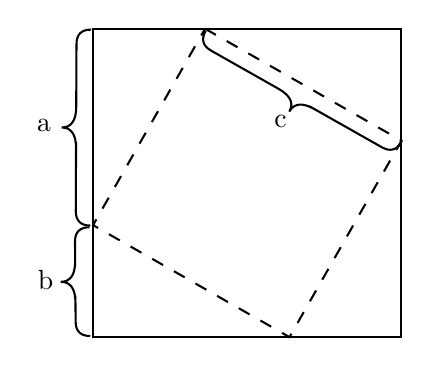
\begin{tikzpicture}[x=0.75pt,y=0.75pt,yscale=-1,xscale=1]

		\tikzset{every picture/.style={line width=0.75pt}} %set default line width to 0.75pt  

		%uncomment if require: \path (0,267); %set diagram left start at 0, and has height of 267

		%Shape: Square [id:dp720027489053255] 
		\draw  [color={rgb, 255:red, 0; green, 0; blue, 0 }  ,draw opacity=1 ][fill={rgb, 255:red, 255; green, 255; blue, 255 }  ,fill opacity=1 ][dash pattern={on 4.5pt off 4.5pt}] (143.69,70.36) -- (238.32,124.31) -- (184.37,218.95) -- (89.73,164.99) -- cycle ;
		%Shape: Brace [id:dp5461547793865589] 
		\draw  [line width=0.75]  (143.98,71.4) .. controls (141.69,75.46) and (142.57,78.64) .. (146.63,80.94) -- (179.02,99.27) .. controls (184.83,102.55) and (186.58,106.22) .. (184.28,110.28) .. controls (186.58,106.22) and (190.63,105.83) .. (196.43,109.12)(193.82,107.64) -- (228.83,127.45) .. controls (232.89,129.74) and (236.07,128.86) .. (238.37,124.8) ;
		%Shape: Rectangle [id:dp39435523517532367] 
		\draw   (89.88,70.5) -- (238.18,70.5) -- (238.18,218.8) -- (89.88,218.8) -- cycle ;
		%Shape: Brace [id:dp06296583129727029] 
		\draw   (88.77,70.8) .. controls (84.1,70.78) and (81.76,73.1) .. (81.74,77.77) -- (81.61,107.97) .. controls (81.58,114.64) and (79.24,117.96) .. (74.57,117.94) .. controls (79.24,117.96) and (81.56,121.3) .. (81.53,127.97)(81.54,124.97) -- (81.4,158.17) .. controls (81.38,162.84) and (83.7,165.18) .. (88.37,165.2) ;
		%Shape: Brace [id:dp8263577400071778] 
		\draw   (87.97,166) .. controls (83.3,166.03) and (80.99,168.38) .. (81.02,173.05) -- (81.09,182.25) .. controls (81.14,188.92) and (78.84,192.27) .. (74.17,192.31) .. controls (78.84,192.27) and (81.19,195.58) .. (81.24,202.25)(81.22,199.25) -- (81.32,211.45) .. controls (81.35,216.12) and (83.7,218.43) .. (88.37,218.4) ;

		% Text Node
		\draw (180.03,115) node  [align=left] {c};
		% Text Node
		\draw (66,117.2) node  [align=left] {a};
		% Text Node
		\draw (66.8,191.2) node  [align=left] {b};


	\end{tikzpicture}
\end{center}

\end{multicols}

Como $A=A$ podemos igualar as duas expressões:

\begin{gather*}
	(a+b)^2=\frac{4}{2}\cdot ab+c^2\\
	a^2+2ab+b^2=2ab+c^2\\
	a^2+\cancel{2ab}+b^2=\cancel{2ab}+c^2\\
	\boxed{a^2+b^2=c^2}
\end{gather*}

\section{\texorpdfstring{$\sen\alpha$ e $\cos\alpha$}{sen a e cos a}}

Se pegarmos um ângulo $\alpha$ de um triângulo retângulo (que não seja o ângulo reto), podemos definir duas medidas básicas a partir deste:

\vskip1em

\begin{romanlistinline}
	\item O seno (denotado $\sen \alpha$) e
	\item o cosseno (denotado $\cos \alpha$).
\end{romanlistinline}

\vskip1em

\begin{minipage}{\textwidth}
	\begin{multicols}{2}
		O seno do ângulo será definido como:

		$$
			\sen \alpha = \frac{\textcolor{blue}{CO}}{\textcolor{red}{H}}
		$$

		%\nopagebreak

		Onde \textcolor{blue}{$CO$} é o cateto oposto ao ângulo e \textcolor{red}{$H$} é a hipotenusa do triângulo.

		\vskip1em

		O cosseno do ângulo será definido como:

		$$
			\cos \alpha = \frac{\textcolor{blue}{CA}}{\textcolor{red}{H}}
		$$

		Onde \textcolor{blue}{$CA$} é o cateto adjacente (próximo) ao ângulo e \textcolor{red}{$H$} é a hipotenusa do triângulo.

		\columnbreak
		\hskip5em
		\begin{tikzscale}[0.8]
			\tkzDefPoints{0/0/A,4/0/B,4/3/C}
			\tkzDrawSegment[blue](B,C)
			\tkzDrawSegment(A,B)
			\tkzDrawSegment[red](A,C)

			\tkzLabelSegment[right=2pt, blue](B,C){$CO$}
			\tkzLabelSegment[above left, red](A,C){$H$}

			\tkzMarkRightAngle[line width=0.3pt](A,B,C)
			\tkzLabelAngle[pos=0.15](A,B,C){\small$\cdot$}

			\tkzMarkAngle[size=1](B,A,C)
			\tkzLabelPoint[xshift=0.71cm, yshift=14pt](A){$\alpha$}

		\end{tikzscale}
		\vskip5em
		\hskip5em
		\begin{tikzscale}[0.8]
			\tkzDefPoints{0/0/A,4/0/B,4/3/C}
			\tkzDrawSegment(B,C)
			\tkzDrawSegment[blue](A,B)
			\tkzDrawSegment[red](A,C)

			\tkzLabelSegment[below=2pt, xshift=5pt, blue](A,B){$CA$}
			\tkzLabelSegment[above left, red](A,C){$H$}

			\tkzMarkRightAngle[line width=0.3pt](A,B,C)
			\tkzLabelAngle[pos=0.15](A,B,C){\small$\cdot$}

			\tkzMarkAngle[size=1](B,A,C)
			\tkzLabelPoint[xshift=0.71cm, yshift=14pt](A){$\alpha$}

		\end{tikzscale}

	\end{multicols}

\end{minipage}
\vskip1em
\begin{minipage}{\textwidth}

	Podemos notar também que essas razões em função do ângulo não se alteram, independentemente do tamanho dos lados.

	\paragraph{Exemplo:}

	\begin{multicols}{2}

		\begin{gather*}
			\sen\SI{30}{\degree}=\frac{\textcolor{red}{a}}{\textcolor{red}{h}}=\frac{\textcolor{blue}{a'}}{\textcolor{blue}{h'}}=\frac{\textcolor{orange}{a''}}{\textcolor{orange}{h''}}\\
			\cos\SI{30}{\degree}=\frac{\textcolor{red}{b}}{\textcolor{red}{h}}=\frac{\textcolor{blue}{b'}}{\textcolor{blue}{h'}}=\frac{\textcolor{orange}{b''}}{\textcolor{orange}{h''}}
		\end{gather*}

		O valor de $\sen\SI{30}{\degree}$ e $\cos\SI{30}{\degree}$ é o mesmo independente do tamanho do comprimento dos catetos ou da hipotenusa.

		\begin{tikzscale}[0.8]
	\tkzDefPoints{0/0/A,3/0/B,5/0/C,8/0/D}
	\tkzDefPoint(30:9){E}

	\tkzDefLine[perpendicular=through B](A,B) \tkzGetPoint{b}
	\tkzDefLine[perpendicular=through C](A,C) \tkzGetPoint{c}
	\tkzDefLine[perpendicular=through D](A,D) \tkzGetPoint{d}

	\pgfresetboundingbox

	\tkzDefPoints{0/-0.7/AB,0/-1.4/AC,0/-2.1/AD,3/-0.7/B',5/-1.4/C',8/-2.1/D'}

	\tkzDrawSegment[red](AB,B')
	\tkzDrawSegment[blue](AC,C')
	\tkzDrawSegment[orange](AD,D')

	\tkzInterLL(A,E)(B,b) \tkzGetPoint{I1}
	\tkzInterLL(A,E)(C,c) \tkzGetPoint{I2}
	\tkzInterLL(A,E)(D,d) \tkzGetPoint{I3}

	\begin{scope}[rotate=30]
		\tkzDefPoints{0/0.7/AI1,0/1.4/AI2,0/2.1/AI3}

		\foreach \i in {1, 2, 3}{
				\begin{scope}[shift={(I\i)}]
					\tkzDefPoint(0, 0.7*\i){I\i '}
				\end{scope}
			}
	\end{scope}

	\tkzDrawSegment[red](AI1,I1')
	\tkzDrawSegment[blue](AI2,I2')
	\tkzDrawSegment[orange](AI3,I3')

	\tkzLabelSegment[below, rotate=30, red](AI1,I1'){$h$}
	\tkzLabelSegment[below, rotate=30, blue](AI2,I2'){$h'$}
	\tkzLabelSegment[below, rotate=30, orange](AI3,I3'){$h''$}

	\tkzDrawLines[add=0 and 0.1 ,style=dashed](A,AI3 I1,I1' I2,I2' I3,I3')

	\tkzDrawLine[add=0 and 0.2](A,D)
	\tkzDrawLine[add=0 and 0.2](A,E)

	\tkzMarkAngle[size=1](B,A,I1)
	\tkzLabelPoint[xshift=0.71cm, yshift=14pt](A){$\SI{30}{\degree}$}

	\tkzMarkRightAngle[line width=0.3pt](A,B,I1)
	\tkzLabelAngle[pos=0.15](A,B,I1){\small$\cdot$}

	\tkzMarkRightAngle[line width=0.3pt](A,C,I2)
	\tkzLabelAngle[pos=0.15](A,C,I2){\small$\cdot$}

	\tkzMarkRightAngle[line width=0.3pt](A,D,I3)
	\tkzLabelAngle[pos=0.15](A,D,I3){\small$\cdot$}

	\tkzDrawSegment[red](B,I1)
	\tkzDrawSegment[blue](C,I2)
	\tkzDrawSegment[orange](D,I3)

	\tkzLabelSegment[right, red](B,I1){$a$}
	\tkzLabelSegment[right, blue](C,I2){$a'$}
	\tkzLabelSegment[right, orange](D,I3){$a''$}

	\tkzLabelSegment[above, red](AB,B'){$b$}
	\tkzLabelSegment[above, blue](AC,C'){$b'$}
	\tkzLabelSegment[above, orange](AD,D'){$b''$}

	\tkzDrawLines[add=0 and 0.1 ,style=dashed](A,AD B,B' C,C' D,D')

	\tkzDrawPoints(B,C,D,I1,I2,I3)

\end{tikzscale}

	\end{multicols}
\end{minipage}

\section{\texorpdfstring{$\tg\alpha$ e $\cotg\alpha$}{tg a e cotg a}}

\begin{minipage}{\textwidth}
	\begin{multicols}{2}
		\noindent Temos também a tangente (denotada $\tg \alpha$), que será a relação:
		\begin{align*}
			\tg\alpha & = \frac{\sen\alpha}{\cos\alpha}                        \\
			          & = \dfrac{\frac{CO}{H}}{\frac{CA}{H}}                   \\
			          & = \dfrac{\frac{CO}{\cancel{H}}}{\frac{CA}{\cancel{H}}} \\
			\tg\alpha & = \frac{\textcolor{blue}{CO}}{\textcolor{red}{CA}}
		\end{align*}
		\noindent E sua recíproca, a cotangente (denotada $\cotg\alpha$):
		$$
			\cotg\alpha=\frac{1}{\tg\alpha}=\frac{\cos\alpha}{\sen\alpha}=\frac{\textcolor{red}{CA}}{\textcolor{blue}{CO}}
		$$
		\begin{tikzscale}[0.8]
			\tkzDefPoints{0/0/A,4/0/B,4/3/C}
			\tkzDrawSegment[red](A,B)
			\tkzDrawSegment[blue](B,C)
			\tkzDrawSegment(A,C)

			\tkzLabelSegment[below=2pt, xshift=5pt, red](A,B){$CA$}
			\tkzLabelSegment[right, blue](B,C){$CO$}

			\tkzMarkRightAngle[line width=0.3pt](A,B,C)
			\tkzLabelAngle[pos=0.15](A,B,C){\small$\cdot$}

			\tkzMarkAngle[size=1](B,A,C)
			\tkzLabelPoint[xshift=0.71cm, yshift=14pt](A){$\alpha$}

		\end{tikzscale}
	\end{multicols}
\end{minipage}

\section{Relações básicas entre razões}

Dizemos que dois ângulos quaisquer $\alpha$ e $\beta$ são complementares se sua soma resulta em $\SI{90}{\degree}$.

Sabemos que a soma dos ângulos de um triângulo qualquer é $\SI{180}{\degree}$ (medida conhecida como "ângulo raso").

Como um triângulo retângulo sempre terá um ângulo reto, os que sobram devem somar $\SI{90}{\degree}$, e, portanto, serão sempre complementares.

Dado um triângulo retângulo $ABC$ qualquer

\begin{multicols}{2}
	\begin{gather*}
		\alpha + \beta + \SI{90}{\degree}=\SI{180}{\degree}\\
		\alpha + \beta = \SI{90}{\degree}
	\end{gather*}

	\vfill\null
	\columnbreak

	\begin{tikzscale}[0.8]
		\tkzDefPoints{0/0/A,4/0/B,4/3/C}
		\tkzDrawTriangle[pythagore](A,B)

		\tkzMarkRightAngle[line width=0.3pt](A,B,C)
		\tkzLabelAngle[pos=0.15](A,B,C){\small$\cdot$}

		\tkzMarkAngle[size=1](B,A,C)
		\tkzLabelPoint[xshift=0.71cm, yshift=14pt](A){$\alpha$}

		\tkzMarkAngle[size=0.8](A,C,B)
		\tkzLabelPoint[xshift=-18pt, yshift=-15pt](C){$\beta$}
	\end{tikzscale}
\end{multicols}

Dado que dois ângulos $\alpha$ e $\beta$ são complementares, podemos verificar que

$$
	\sen \alpha=\frac{a}{b}=\cos\beta
$$

e o contrário ($\cos\alpha=\sen\beta$) também se verifica.

Outra relação que surge dessa é que

$$
	\tg\alpha=\frac{\sen\alpha}{\cos\alpha}=\frac{\cos\beta}{\sen\beta}=\cotg\beta
$$

naturalmente, também vale que $\tg\beta=\cotg\alpha$.

\section{Relação fundamental da trigonometria}

\begin{minipage}{\textwidth}
	Aplicando o teorema de pitágoras em um triângulo retângulo $ABC$ qualquer, temos que:
	\nopagebreak
	\begin{multicols}{2}
		\begin{gather*}
			a^2+b^2=c^2\\
			\frac{a^2}{c^2}+\frac{b^2}{c^2}=\frac{\cancel{c^2}}{\cancel{c^2}}\\
			\left(\vphantom{\dfrac{b}c}\dfrac{a}c\right)^2 +\left(\frac{b}{c}\right)^2=1\\
			(\sen \alpha)^2+(\cos \alpha)^2=1\\
			\boxed{\sen^2 \alpha + \cos^2 \alpha=1}
		\end{gather*}
		\vfill\null
		\columnbreak
		\vfill\null
		\begin{tikzscale}[0.8]
			\tkzDefPoints{0/0/A,4/0/B,4/3/C}
			\tkzDrawTriangle[pythagore](A,B)

			\tkzLabelSegment[below=2pt, xshift=3pt](A,B){$b$}
			\tkzLabelSegment[right=2pt, yshift=-2pt](B,C){$a$}
			\tkzLabelSegment[above left](A,C){$c$}

			\tkzMarkRightAngle[line width=0.3pt](A,B,C)
		\end{tikzscale}
	\end{multicols}

	A relação fundamental da trigonometria vale para qualquer ângulo $\alpha$.
\end{minipage}

